\documentclass[a4paper,12pt]{article}

\usepackage{natbib}
\usepackage{times}
\usepackage{graphicx,epsfig}
\usepackage[leftcaption]{sidecap}
\usepackage{subfigure} % figures can have sub chunks
\usepackage{geometry} % this maxes page usage, making the below unnecessary
% \textwidth = 6.75in
% \oddsidemargin = -0.25in
% \textheight = 10in
% \topmargin = -0.5in

\textwidth = 7.25in 
\oddsidemargin = -0.5in
\textheight = 10.25in
\topmargin = -0.75in

\usepackage{fancyhdr}
\pagestyle{fancy}
\lhead{{\it Alan Lau}}
\chead{Wall Following LEGO Robots}
\rhead{Coursework 1}
\lfoot{}
\cfoot{\thepage}
\rfoot{}
\usepackage[T1]{fontenc}
\usepackage{multirow}
\usepackage{multicol}
\usepackage{array}
\usepackage{caption}
\usepackage{hyperref}
\usepackage{graphicx}
\graphicspath{ {images/} }

\usepackage{calc}
\setlength{\parskip}{5pt}
\setlength{\parindent}{0pt}
% \addtolength{\hoffset}{0.5cm}
% \addtolength{\textwidth}{0.5cm}

% set section depth
\setcounter{tocdepth}{4}
\setcounter{secnumdepth}{5}

\newcommand{\goodgap}{%
 \hspace{\subfigtopskip}%
 \hspace{\subfigbottomskip}}

\title{Coursework 1:  Wall Following with a LEGO Robot}
\author{Alan Lau}


\begin{document}
\maketitle

\section{Introduction}
We created a LEGO robot capable of navigating around obstacles along a wallside. During the development of the robot, we came up with the following hypothesis:

\begin{center}
    "There is an optimal combination of parameters that yields the fastest time in completing a pre-set course with obstacles for a reactive robot." 
\end{center}

Our aim is to explore how prior knowledge impacts the success of a robot, and attempt to find optimal parameters that gives the fastest lap time. Our experiments show that there is a connection between motor speed and minimum distance between robot and obstacle which affects how the robot complete the course and the number of collisions occur, hence the optimal set of parameters might not give the fastest lap time, but instead, provides the robot with a balanced performance. Our robot design (see \autoref{fig:robot}) centres with the idea of reactivity as described by \cite{brooks1991}. We focus our efforts in making our robot perform actions based on the environment it is in through sensing its surrounding, rather than hard-coding its behaviour around a specific course. However, prior information is also key. One requires the facility to rotate and move forward in order to perform navigation, which motivates us to perform the experiments shown below.

% - hypothesis (what you tried to do)
% - motivation (why you have done that)
% - brief background for arguments
% - cite papers for motivation (e.g. Brooks 1991)
% - present a single hypothesis you tested on your completed robot about how to improve its intelligence

\section{Approach}
Simon Elvin (sje29) and I worked throughout the development of the robot. We created the robot together and pair programmed the logic of our robot. Also, we ran the experiments together. However, we independently interpreted the results in each of our own report.

First, we define some settings for our experiments. We ran our experiments using the the setup found in the MSc laboratory, as illustrated in \autoref{fig:course}. We believe this is a suitable course, as it contains both obvious corners, such as the ones around the black cabinet, and more sutble corners with shorter distances and depth, such as those around the red cabinets and the bin. Also, we define `success' as being able to complete the course by going from the starting point to the end point, where the robot has followed the majority of corners.

We decide to focus our experiments to vary two variables to constraint the test space - \textit{motor speed} and \textit{the minimum distance between the head and an obstacle}. The latter affects other distance measures that are used, such as the distance to which the robot decides it has lost the wall (\texttt{CONVEX\_WALL\_THRESHOLD}). They are formed by adding a fixed value is added to the minimum distance. Similarly, we fix some other parameters, such as the motor rotation factor, which is used to rectify the under-steering caused by the friction against the carpet.

We then carry out our tests, where we start by making the robot to face towards the black cabinet. We recorded the time taken for the robot to complete the course, the number of collisions to the bumper and the back of the robot, and the number of corners missed. As shown in \autoref{tab:exp-config}, we performed tests with combinations of three different speeds and three different minimum distances, for which we obtain three runs per combination. 

% - describe in detail what exactly we have done 
    % - e.g. experiements set up to determine in what conditions you could make better results (replicability) (cite paper)
% - who I partnered with and how much we worked together
% - questions
    % - contrasting the addition of extra control algorithms
    % - changing the physical shape of the robot
    % - trying different target sonar readings for maintaining a particular distance
    % - circuit time, success rate
% - capture, describe the things that makes a difference in performance
% - consider chagning variables - battery, daylight, proximity to other sonar-using robots to explain strange behaviour


\section{Results}
In \autoref{fig:time-avg}, we can see that there is a downward trend in the average time required to complete the course as both the speed of the motor and the minimum distance increases. Test 3-1 and 3-2 lack a standard deviation value as there is only one successful run under each of those settings.

Parameters used in Test 3-3 obtained the fastest lap time, whereas those from Test 1-1 were the slowest. The lap times obtained from Test 2 are significantly faster than those in Test 1 (t-test, p < 0.0019). Also, there is a significant difference between the mean collisions per run, when comparing the results of a minimum distance of 0.2 (Tests 1-1, 2-1, 3-1) and that of 0.4 (Tests 1-3, 2-3, 3-3) (f-test, p < 0.0075). However, the mean of missed corners as the motor speed increases remains unchanged deemed to be not significant under both t-test and f-test.

Interesting observations can be made by focusing on Test 1-3, Test 2-2 and Test 3-3. Both Test 1-3 and 3-3 have a lower average collision per run compared to Test 2-2, but Test 2-2 missed the fewest angles on average. Test 1-3 obtained the slowest lap time of the three tests, while Test 3-3 obtained the fastest. Test 2-2 also has the lowest standard deviation amongst all other tests. This \href{https://goo.gl/photos/G1PmLfxJktHRtpsm6}{\textbf{\textit{link}}} shows the robot in action under the Test 2-2 configuration. 

% - describes the outcome - factual descriptions (qualitative, quantitative)
    % - significance testing & standard deviation - e.g. avg speed around a circuit in two conditions
% - video to prove the conditions lead to different results
% - precise, factual results only - info to be described in approach
% - an insightful comment about one or more cited papers
% supported by evidence from your experience might get you these extra
% marks
% - so might a particularly accurate and replicable account of
% your approach and results


\section{Discussion}
We observe that the combinations of speed and minimum distance have an impact on the number of collisions and success rate. Through examining Test 3-1, we can see that the extreme configuration with a high speed and a small minimum distance did not perform well. The robot failed to complete the course two out of three times, as it approach the wall too quickly so it do not have enough time to rotate. The completed run has the robot colliding with the wall for 13 times and detected no corners. It has the slowest lap time even when compared with the slowest speed settings. Also, as the minimum distance is increased, the robot gradually becomes more prone to less distinguishable angles. In Test 3-3, the runs consistently missed the corners around the bin and the red cabinets (see \autoref{fig:course}).

The results and these observations show that whilst one can solely increase the speed of the robot to achieve a faster lap time, this comes at a cost if other parameters are not tuned properly at the same time. Too small a minimum distance will cause the robot to collide into obstacles constantly; too large will cause the robot to miss subtle corners. Whilst Test 2-2 did not give the fastest speed, it demonstrates its ability to navigate smoothly with minimal collisions and a relatively fast lap time.

To further improve our experiments and results, more runs for each configuration should be performed to obtain more confident results. Further experiments on obstacles made with different materials and different lighting situations could help find a generic set of optimal parameters that works in various indoor situations.

% - include speculation
% - discuss how results address the questions described in intro
% - how restuls imply about your own worka and AI or robotics in general
% - suggest other experiments that might give other insights
% - can be long with comparisons with papers 


\section{Conclusion}
% - on paragraph
% - restate what we tried to do and the outcome
% - results in light of the intro
We show that there is a trade-off between speed and accuracy, hence there is not an optimal set of parameters that gives the fastest lap time. Instead, an optimal set of parameters would act as a balancing act. The parameters from Test 2-2 demonstrates this by making the robot to navigate through the course at a rather good time whilst retaining much of its intelligence and accuracy. 

\newpage
\bibliographystyle{apalike}
\bibliography{biblio}

\appendix
\section{Tables and Graphs}

% TABLE - states and commands
%%%%%%%%%%%%%%%%%%%
{\renewcommand{\arraystretch}{1.3}%
\parbox{\linewidth} {
    \centering
  \begin{tabular}{|m{0.15\textwidth}|m{0.22\textwidth}|m{0.22\textwidth}|m{0.22\textwidth}|}
        \hline

%%%%%%%% States
        %\multirow{3}{*}{%}
    \textbf{States}
      & \texttt{FINDING\_WALL} & \texttt{FOLLOWING\_WALL} & \texttt{LOOKING\_FORWARD}
    \\ \hline
%%%%%%%% States 

%%%%%%%% Commands
    \multirow{6}{*}{\textbf{Commands}}
      & \multicolumn{3}{c|}{\texttt{TOO\_CLOSE}} 
      \\ %\cline{2-4}

      & \multicolumn{3}{c|}{\texttt{TOO\_FAR}} 
      \\ %\cline{2-4}

      & \multicolumn{3}{c|}{\texttt{IN\_RANGE\_FAR}} 
      \\ %\cline{2-4}

      & \multicolumn{3}{c|}{\texttt{IN\_RANGE\_CLOSE}} 
      \\ %\cline{2-4}

      & \multicolumn{3}{c|}{\texttt{INTERVAL\_REACHED}} 
      \\ %\cline{2-4}

      & \multicolumn{3}{c|}{\texttt{TOUCH\_CONTACT}} 
      \\ \hline
%%%%%%%% Commands

    \end{tabular}
\captionof{table}{\textit{States and commands used by the robot.}}
\label{tab:states-commands}
}
%%%%%%%%%%%%%%%%%%%%%%%

\vspace{15mm}

% TABLE - Experiment configurations
%%%%%%%%%%%%%%%%%%%
{\renewcommand{\arraystretch}{1.3}%
\parbox{\linewidth} {
    \centering
  \begin{tabular}{|m{0.1\textwidth}|m{0.25\textwidth}|m{0.25\textwidth}|}
        \hline

%%%%%%%% Header
    \textbf{Test}
      & \textbf{Speed (degrees/sec)} & \textbf{Minimum Distance (m)} 
    \\ \hline
%%%%%%%% Header 

%%%%%%%% Tests 
    Test 1-1 & 200 & 0.2
    \\ \hline

    Test 1-2 & 200 & 0.3
    \\ \hline

    Test 1-3 & 200 & 0.4
    \\ \hline

    Test 2-1 & 400 & 0.2
    \\ \hline

    Test 2-2 & 400 & 0.3
    \\ \hline
      
    Test 2-3 & 400 & 0.4
    \\ \hline

    Test 3-1 & 600 & 0.2
    \\ \hline

    Test 3-2 & 600 & 0.3
    \\ \hline
      
    Test 3-3 & 600 & 0.4
    \\ \hline
%%%%%%%% Commands

    \end{tabular}
\captionof{table}{\textit{The different test parameter combinations. Note that variables depending on the minimum distance, i.e.} \texttt{CONCAVE\_WALL\_THRESHOLD} \textit{and} \texttt{CONVEX\_WALL\_THRESHOLD}.}
\label{tab:exp-config}
}
%%%%%%%%%%%%%%%%%%%%%%%



% TABLE - Experiment info
%%%%%%%%%%%%%%%%%%%
{\renewcommand{\arraystretch}{1.3}%
\parbox{\linewidth} {
    \centering
    \begin{tabular}{|m{0.1\textwidth}|m{0.2\textwidth}|m{0.2\textwidth}|m{0.25\textwidth}|m{0.1\textwidth}|}
        \hline

%%%%%%%% Header
        \textbf{Test} & \textbf{Mean time (sec)} & \textbf{Mean collisions / run} & \textbf{Mean missed corners / run} & \textbf{Success rate (\%)}
        \\ \hline
%%%%%%%% Header 

%%%%%%%% Averages 
        Test 1-1 & 139.86 & 1.67 & 0.33 & 100\%
        \\ \hline

        Test 1-2 & 129.63 & 1 & 0.67 & 100\%
        \\ \hline

        Test 1-3 & 125.5 & 0.33 & 1.4 & 100\%
        \\ \hline

        Test 2-1 & 88.83 & 6.67 & 0.67 & 100\%
        \\ \hline

        Test 2-2 & 70.18 & 2 & 0.67 & 100\%
        \\ \hline
          
        Test 2-3 & 69.63 & 0.5 & 1 & 100\%
        \\ \hline

        \textit{Test 3-1} & \textit{143.52} & \textit{13} & \textit{0} & \textit{33.30\%}
        \\ \hline

        \textit{Test 3-2} & \textit{48.57} & \textit{0} & \textit{3} & \textit{33.30\%}
        \\ \hline
          
        Test 3-3 & 50.35 & 1 & 2.67 & 100\%
        \\ \hline
%%%%%%%% Averages 

    \end{tabular}
\captionof{table}{\textit{Mean metrics of the experiment results. Note that Test 3-1 and Test 3-2 each only has one successful run out of three, so these are the values obtained for the successful run, rather than an average.}}
\label{tab:exp-info}
}
%%%%%%%%%%%%%%%%%%%%%%%

\vspace{10mm}

% FIG - navigation course 
\begin{figure}[h]
    \centering
    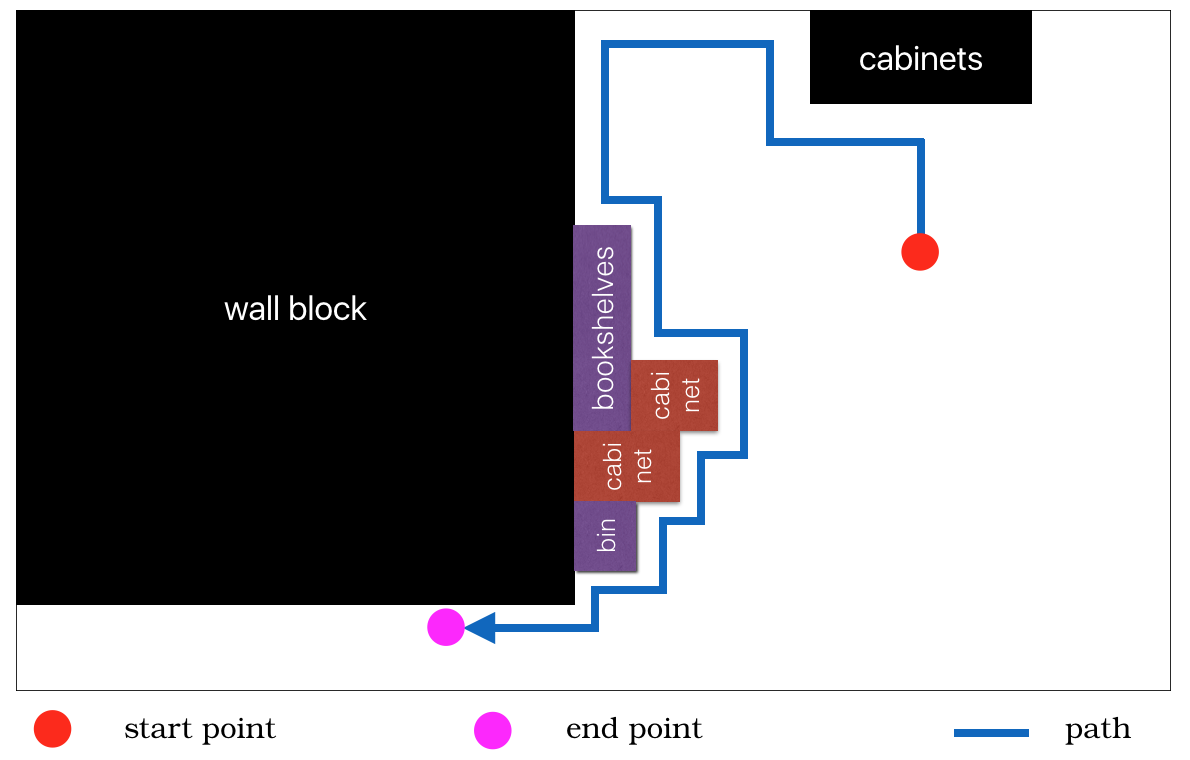
\includegraphics[width=0.8\textwidth]{path}
    \caption{\textit{A bird's-eye view of the course setup used to develop and test the robot against our hypothesis.}}
    \label{fig:course}
\end{figure}

% FIG - test average time 
\begin{figure}[h]
    \centering
    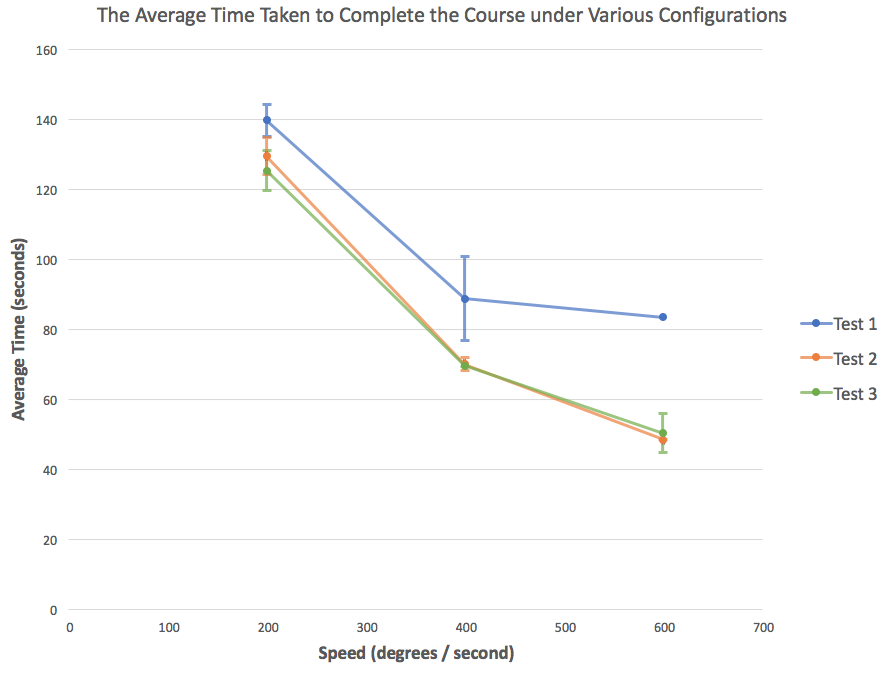
\includegraphics[width=0.8\textwidth]{time-avg}
    \caption{\textit{We plot the average value out of the three runs, and the standard deviation bar using the sample for each configuration. Some configurations, namely, Test 1-3 and Test 3-2, failed on one or more test runs, hence a standard deviation bar is not available.}}
    \label{fig:time-avg}
\end{figure}

% FIG - robot
\begin{figure}[h]
    \centering
    \includegraphics[width=0.8\textwidth]{robot}
    \caption{\textit{Our robot design - a sonar sensor (`head') is attached to a motor which enables a 180-degree view (looking forward, right and left), and is mounted at a high position to capture big obstacles. Two touch sensors (`bumper') are attached in a lower position to detect low-lying obstacles and collisions. The intelligence relies heavily on the readings from the head, as we view collision as unintelligent and should be avoided. Our robot can be more intelligent by alter the motor speed if we detect that there is a wall ahead and closely monitor the wall in front and turn in time. Also, more sensors, such as a gyroscope can be used to detect the rotation angle so that a hard-coded rotation factor will not be required. }}
    \label{fig:robot}
\end{figure}

\end{document}
